% Anexo con las baterías y la robustez de detalle del Capítulo de resultados (movidas desde 04_resultados.tex).
\chapter{Baterías y robustez detallada}
\label{chap:anexo-robustez}

Este anexo reúne las tablas y figuras de detalle del Capítulo~\ref{sec:resultados}: las dos baterías de regresiones, las figuras de robustez de la interacción y las secciones de robustez a la medición, a la muestra y a la forma funcional, que el capítulo resume en la Sección~\ref{sec:robustez-resumen}.

\section{Baterías de regresiones}
\label{sec:anexo-baterias}

La Tabla~\ref{tab:bateria-lnlag-embiext} reúne 36 regresiones: cuatro modelos anidados por tres estructuras de efectos fijos por tres muestras. La columna (1) del Panel A es la regresión principal, la ecuación~\eqref{eq:principal} sin controles con efectos fijos de país y de tiempo, que la Tabla~\ref{tab:principal-compacta} reproduce. Las Tablas~\ref{tab:crisis-lnlag-embiext} y~\ref{tab:crisis-lnlag-embiext-b} estiman la interacción con el vector de crisis (Sección~\ref{sec:crisis-interaccion}).

\input{\tablasdir/tablas_regresiones_lnlag_embiext_t1}

\input{\tablasdir/tablas_regresiones_lnlag_embiext_t2}

\section{Figuras de robustez de la interacción}
\label{sec:anexo-figuras}

Las figuras de esta sección acompañan a las Secciones~\ref{sec:magnitud-nolineal}, \ref{sec:niveles-logs}, \ref{sec:robustez-interaccion} y~\ref{sec:crisis-interaccion}.

\begin{figure}[htbp]
\centering
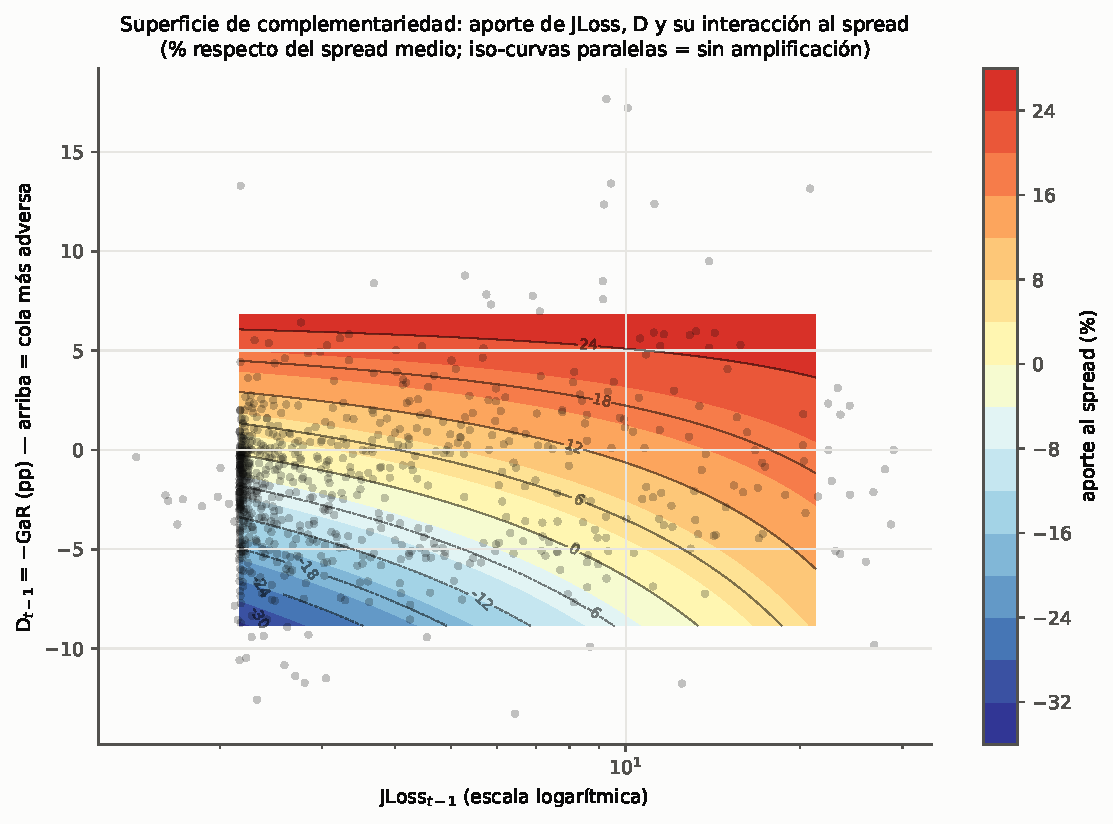
\includegraphics[width=0.82\textwidth]{fig_superficie_lnlag.pdf}
\caption[Superficie de complementariedad]{Aporte de $\ln JLoss_{t-1}$, $D_{t-1}$ y su interacción al spread (en \% respecto del spread medio), regresión principal. Puntos: observaciones.}
\label{fig:superficie}
\end{figure}

\begin{figure}[htbp]
\centering
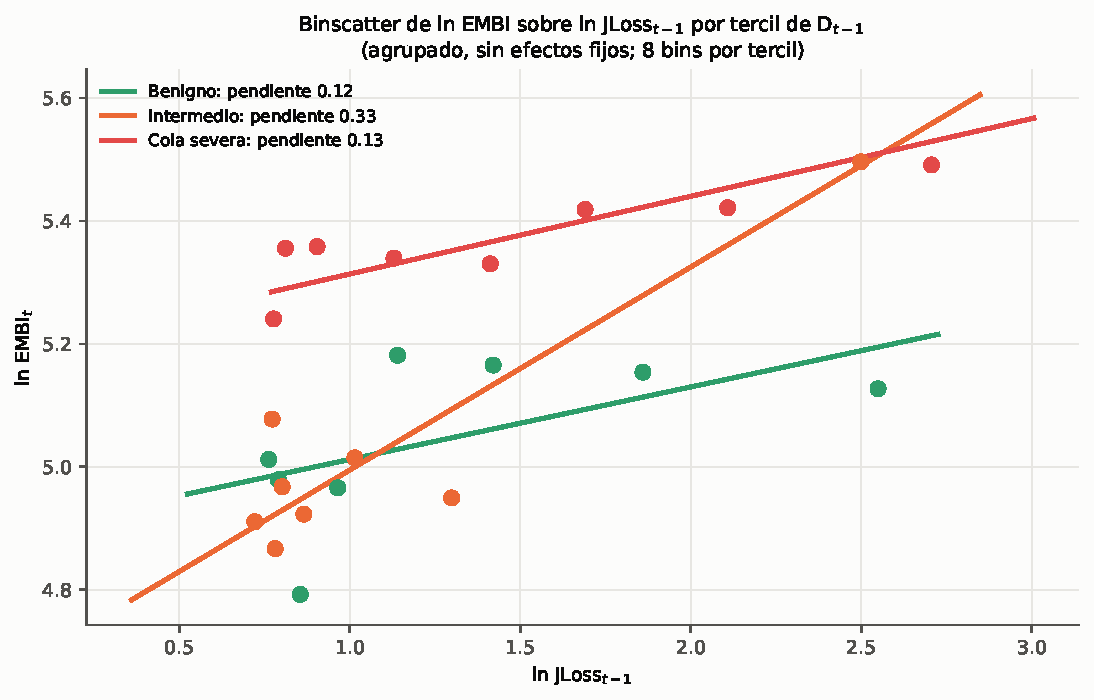
\includegraphics[width=0.78\textwidth]{fig_binscatter_lnlag.pdf}
\caption[\textit{Binscatter} por régimen de riesgo de cola]{\textit{Binscatter} de $\ln$ EMBI sobre $\ln JLoss_{t-1}$ por tercil de $D_{t-1}$ (agrupado, sin efectos fijos; ocho bins por tercil) y recta de MCO por tercil.}
\label{fig:binscatter}
\end{figure}

\begin{figure}[htbp]
\centering
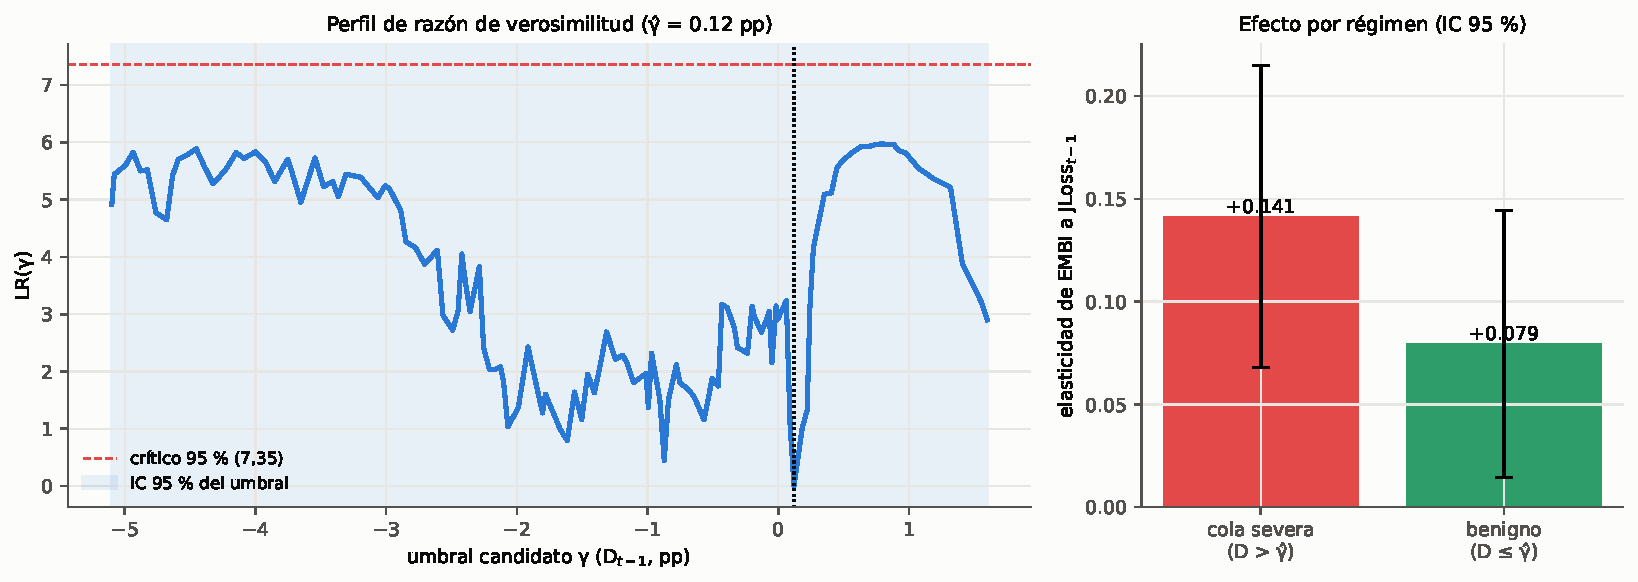
\includegraphics[width=\textwidth]{fig_umbral_lnlag.pdf}
\caption[Modelo de umbral de Hansen]{Modelo de umbral \citep{Hansen2000} en logaritmos. Izquierda: perfil del estadístico $LR(\gamma)$, umbral estimado e IC 95\%. Derecha: elasticidad del spread a $JLoss_{t-1}$ en cada régimen (IC 95\%, Driscoll--Kraay).}
\label{fig:umbral}
\end{figure}

\begin{figure}[htbp]
\centering
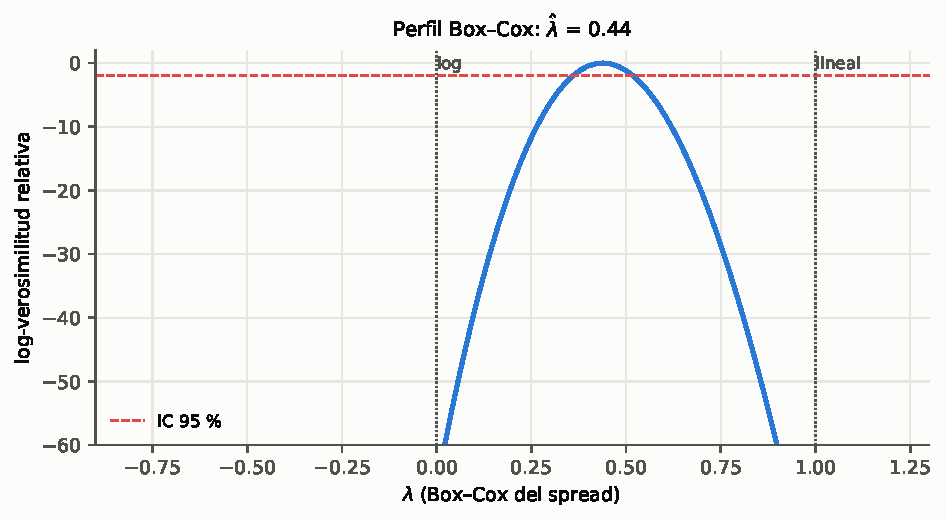
\includegraphics[width=0.72\textwidth]{fig_boxcox_arb.pdf}
\caption[Perfil de Box--Cox]{Log-verosimilitud concentrada de la transformación de Box--Cox del spread, con los regresores de la especificación principal y efectos fijos de país y de tiempo. Línea discontinua: umbral del IC 95\%.}
\label{fig:boxcox}
\end{figure}

\begin{figure}[htbp]
\centering
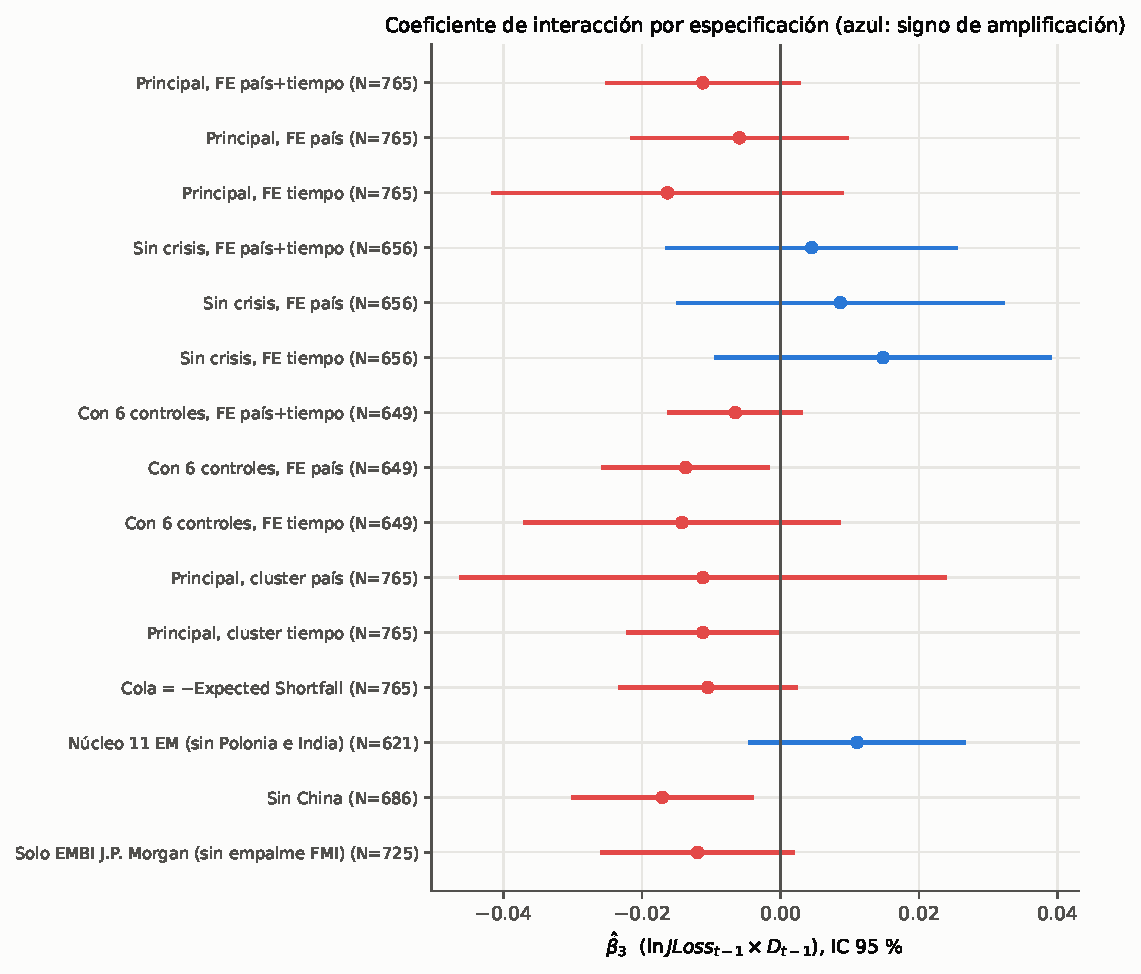
\includegraphics[width=0.85\textwidth]{fig_forest_lnlag.pdf}
\caption[Coeficiente de interacción por especificación]{Coeficiente de interacción $\hat\beta_3$ por especificación, con IC 95\% (Driscoll--Kraay salvo indicación). Azul: signo de amplificación; rojo: signo opuesto.}
\label{fig:forest}
\end{figure}

\begin{figure}[htbp]
\centering
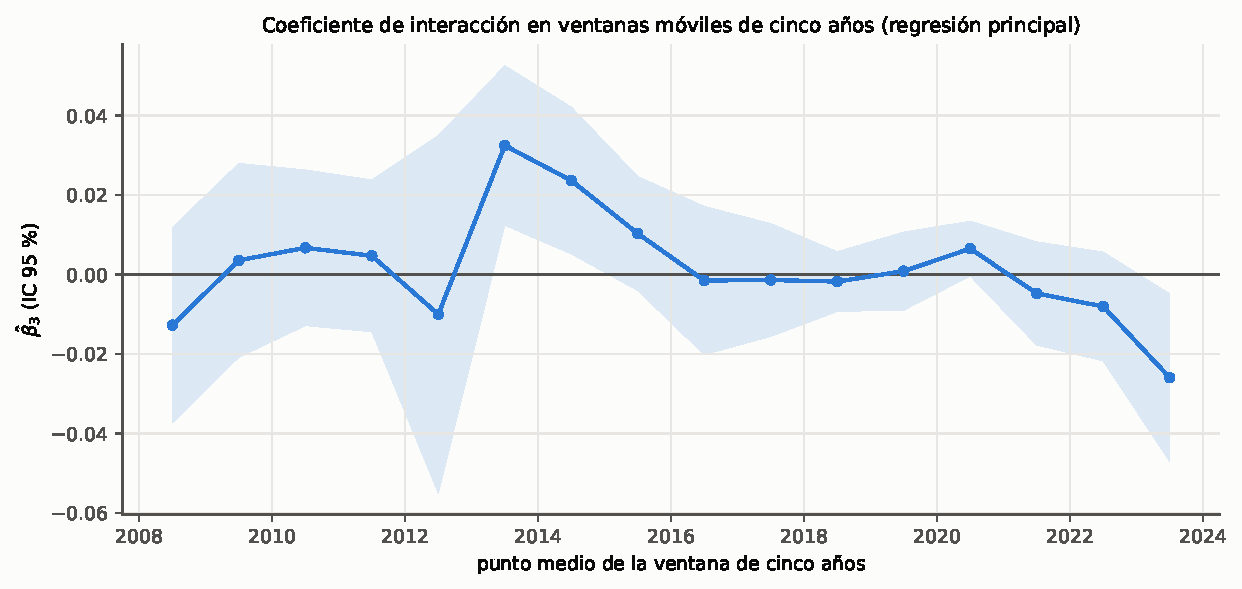
\includegraphics[width=0.85\textwidth]{fig_ventanas_lnlag.pdf}
\caption[Interacción en ventanas móviles]{Coeficiente de interacción de la regresión principal en ventanas móviles de cinco años (IC 95\%). El eje horizontal marca el punto medio de la ventana.}
\label{fig:ventanas}
\end{figure}

\begin{figure}[htbp]
\centering
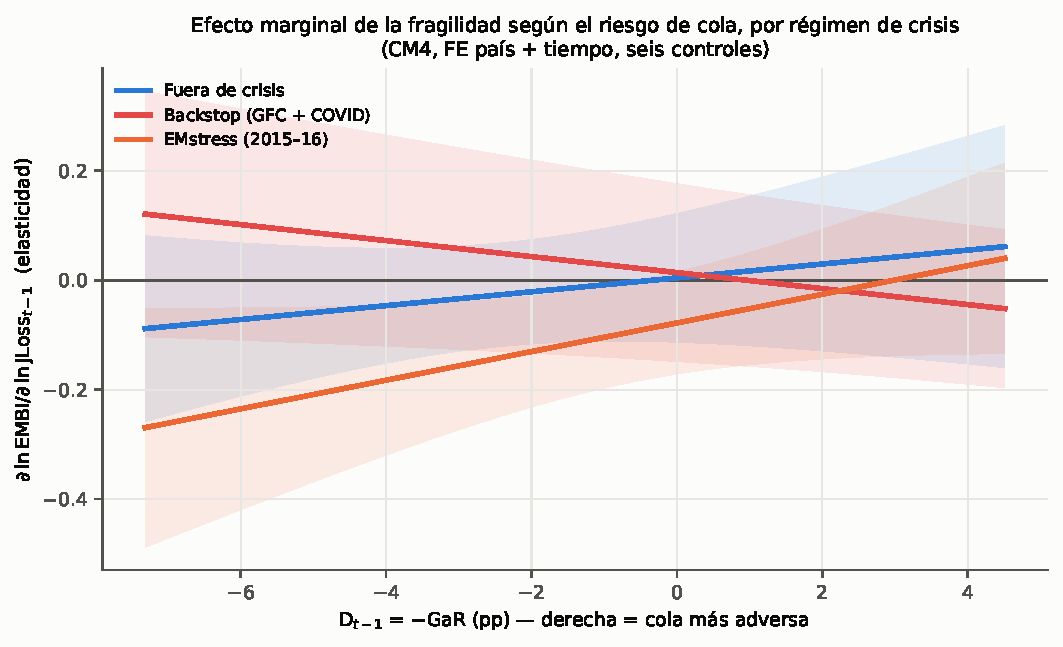
\includegraphics[width=0.85\textwidth]{fig_crisis_regimen_lnlag.pdf}
\caption[Efecto marginal por régimen de crisis]{Elasticidad del spread a $JLoss_{t-1}$ en función de $D_{t-1}$, por régimen (CM4 de la Tabla~\ref{tab:crisis-lnlag-embiext-b}, efectos fijos de país y de tiempo, seis controles). Banda: IC 95\% (Driscoll--Kraay).}
\label{fig:crisisregimen}
\end{figure}

\section{Robustez a la medición y a la muestra}
\label{sec:robustez}

\textbf{Medición de la fragilidad.} Como la cota de la malla de pérdidas es activa en casi todas las observaciones y la métrica tiene un piso (Sección~\ref{sec:magnitud}), $JLoss$ es una medida ordinal. Reemplazando $\ln JLoss_{t-1}$ por su percentil en la muestra, la asociación de la fragilidad se mantiene con Driscoll--Kraay ($0{,}27$ por cada 100 percentiles, $p=0{,}002$; \textit{wild bootstrap}, $0{,}15$), y lo mismo con su valor estandarizado dentro de cada país ($0{,}048$ por desviación estándar, $p=0{,}023$; \textit{wild bootstrap}, $0{,}18$). Recalculando la métrica con una malla más ancha, que correlaciona 0,80 con la base en logaritmos, la elasticidad cae a $0{,}067$ y deja de ser significativa ($p=0{,}22$). La asociación descansa, por tanto, en el ordenamiento de la fragilidad más que en su nivel, y es sensible a la calibración del motor.

\textbf{La fragilidad sin saturación: la probabilidad de incumplimiento de Merton.} Si la componente inesperada de $JLoss$ satura casi siempre, su variación la gobierna la pérdida esperada, es decir, las probabilidades de incumplimiento de Merton ponderadas por exposición. Se puede medir entonces la fragilidad directamente, con el mismo motor y los mismos bancos, de dos formas que no tienen techo ni piso: la probabilidad de incumplimiento media del sistema ponderada por pasivos ($PD_w$, en \%) y menos la distancia al incumplimiento media ($-DD_w$, con $DD=-\Phi^{-1}(PD)$; un valor mayor indica más fragilidad). La Tabla~\ref{tab:fragilidad-alternativa} reestima la regresión principal con cada una. Las dos correlacionan con $\ln JLoss_{t-1}$ ($0{,}71$ y $0{,}85$) y entregan la misma magnitud por desviación estándar dentro del país: un spread entre un 5\% y un 8\% mayor, o unos 18 puntos básicos. Pero la asociación es más nítida, en especial con la distancia al incumplimiento: en logaritmos su $p$ de \textit{wild bootstrap} es $0{,}055$ (con errores agrupados, $0{,}044$), frente a $0{,}32$ con $JLoss$, y en puntos básicos es $0{,}048$. La interacción, en cambio, sigue siendo nula en logaritmos con las tres medidas ($p$ de \textit{wild bootstrap} entre $0{,}89$ y $0{,}997$). En puntos básicos es positiva con la distancia al incumplimiento ($1{,}87$; $p=0{,}017$ con Driscoll--Kraay, $0{,}13$ con \textit{wild bootstrap}), que es lo que implica la estructura multiplicativa del marco teórico (Sección~\ref{sec:sintesis-pilares}) y no amplificación. La saturación de $JLoss$ atenúa, por tanto, la asociación de la fragilidad con el spread; no explica la ausencia de amplificación. Como estas medidas no estaban preespecificadas y no se sometieron a la exclusión de cada país, se califican de sugerentes.

\begin{table}[htbp]
\centering
\small
\caption[Fragilidad sin saturación]{La regresión principal con medidas de fragilidad que no saturan}
\label{tab:fragilidad-alternativa}
\begin{adjustbox}{max width=\linewidth}
\begin{tabular}{l cccc}
\toprule
 & $\ln JLoss$ (base) & $\ln PD_w$ & $-DD_w$ & $\ln JLoss$, malla ancha \\
\midrule
\multicolumn{5}{l}{\textit{A. Logaritmos: $\ln$ EMBI}} \\
\quad Fragilidad ($\beta_1$) & $0{,}099^{***}$ & $0{,}021^{***}$ & $0{,}082^{***}$ & $0{,}067$ \\
\quad \quad $p$: \textit{cluster} / \textit{wild} & $0{,}28$ / $0{,}32$ & $0{,}075$ / $0{,}091$ & $0{,}044$ / $0{,}055$ & $0{,}47$ / $0{,}47$ \\
\quad \quad por d.e. dentro del país & $0{,}052$ & $0{,}057$ & $0{,}080$ & $0{,}031$ \\
\quad Riesgo de cola ($\beta_2$) & $0{,}032^{**}$ & $0{,}031^{*}$ & $0{,}029^{*}$ & $0{,}031^{*}$ \\
\quad Interacción ($\beta_3$) & $-0{,}011$ & $0{,}0005$ & $0{,}0001$ & $0{,}002$ \\
\quad \quad $p$ \textit{wild} & $0{,}90$ & $0{,}89$ & $0{,}997$ & $0{,}99$ \\
\addlinespace
\multicolumn{5}{l}{\textit{B. Niveles: EMBI en puntos básicos}} \\
\quad Fragilidad ($\gamma_1$) & $4{,}73^{***}$ & $2{,}14^{***}$ & $18{,}8^{***}$ & $4{,}10^{***}$ \\
\quad \quad $p$ \textit{wild} & $0{,}31$ & $0{,}30$ & $0{,}048$ & $0{,}27$ \\
\quad \quad por d.e. dentro del país (pb) & $18{,}3$ & $18{,}4$ & $18{,}5$ & $19{,}0$ \\
\quad Interacción ($\gamma_3$) & $0{,}25$ & $0{,}11$ & $1{,}87^{**}$ & $0{,}49^{**}$ \\
\quad \quad $p$ \textit{wild} & $0{,}47$ & $0{,}47$ & $0{,}13$ & $0{,}20$ \\
\addlinespace
Correlación con $\ln JLoss_{t-1}$ & $1$ & $0{,}71$ & $0{,}85$ & $0{,}80$ \\
Observaciones (economías) & 765 (13) & 765 (13) & 765 (13) & 710 (12) \\
\bottomrule
\end{tabular}
\end{adjustbox}
\par\smallskip\parbox{0.95\linewidth}{\footnotesize \textit{Nota:} Regresión principal con la medida de fragilidad indicada, rezagada un trimestre y centrada; efectos fijos de país y de tiempo. $PD_w$: probabilidad de incumplimiento de Merton/KMV media del sistema, ponderada por pasivos, en \%; $DD_w$: distancia al incumplimiento media ponderada por pasivos; ambas con el mismo motor y los mismos bancos que $JLoss$. En el Panel B la medida entra sin logaritmo. La malla ancha ($[0{,}01;\,0{,}20]$) no se calculó para India; sobre la misma muestra sin India, la base da $0{,}087$ ($p=0{,}035$; \textit{wild bootstrap}, $0{,}42$). Estrellas según Driscoll--Kraay; \textit{wild cluster bootstrap} por país con pesos de Webb y 999 réplicas. ***, ** y * indican significancia al 1\%, 5\% y 10\%. Fuente: \texttt{p34\_fragilidad\_alternativa.py}.}
\end{table}

\textbf{Composición de la muestra.} Nada cambia al excluir las 40 observaciones de EMBI empalmadas del FMI ($\hat\beta_1=0{,}086$, $\hat\beta_2=0{,}035$, $\hat\beta_3=-0{,}012$), los trimestres en que la métrica se calcula con pocos bancos ($0{,}099$, $0{,}034$ y $-0{,}010$) o al empezar la muestra en 2010 ($0{,}083$, $0{,}037$ y $-0{,}011$).

\textbf{Panel de historia larga.} El panel es desbalanceado: Filipinas aporta doce trimestres, e Indonesia y Sudáfrica treinta y dos, veinte de ellos con el EMBI empalmado. Sobre las diez economías de historia larga ($N=689$) los coeficientes son los de la regresión principal: $0{,}087$ para la fragilidad ($p=0{,}013$), $0{,}035$ para el riesgo de cola ($p=0{,}029$) y $-0{,}012$ para la interacción ($p=0{,}09$); en puntos básicos, $4{,}6$ ($p<0{,}001$), $3{,}7$ ($p=0{,}23$) y $0{,}23$. Los resultados no dependen de las tres economías de cobertura corta. Tampoco cambia la inferencia con pocos \textit{clusters}: con diez países el \textit{wild cluster bootstrap} da $p=0{,}39$ para la fragilidad y $0{,}16$ para el riesgo de cola.

\textbf{Incorporación de Argentina.}\label{sec:robustez-argentina} Argentina tiene el spread más alto y volátil de las economías candidatas ---más de 3.000 puntos básicos en 2020Q2---, de modo que su exclusión podría estar atenuando la asociación entre fragilidad y spread. Se reestimaron las Tablas~\ref{tab:bateria-lnlag-embiext} y~\ref{tab:crisis-lnlag-embiext} añadiéndola al panel: catorce economías y 799 observaciones en la regresión principal. Su EMBI proviene de la serie de subíndices J.P.\ Morgan EMBI Global Diversified (la misma familia que el resto del panel, verificada contra Brasil y México con correlación 0,99999), sus controles del FMI y el Banco Mundial, y su $GaR$ hereda la salvedad descrita en la Sección~\ref{sec:datos}. La Tabla~\ref{tab:argentina} resume la comparación; las tablas completas están en el anexo (Tablas~\ref{tab:bateria-lnlag-embiext-arg} y~\ref{tab:crisis-lnlag-embiext-arg}).

\begin{table}[htbp]
\centering
\small
\caption[Robustez: incorporación de Argentina]{Especificación principal con y sin Argentina (M4, efectos fijos de país y de tiempo, errores de Driscoll--Kraay).}
\label{tab:argentina}
\begin{adjustbox}{max width=\linewidth}
\begin{tabular}{l cc}
\toprule
 & Sin Argentina (13 países) & Con Argentina (14 países) \\
\midrule
\multicolumn{3}{l}{\textit{Muestra completa}} \\
\quad $\ln JLoss_{t-1}$ ($\beta_1$) & $0{,}0985^{***}$ & $0{,}0964^{***}$ \\
\quad $D_{t-1}$ ($\beta_2$) & $0{,}0324^{**}$ & $0{,}0326^{**}$ \\
\quad $\ln JLoss_{t-1}\times D_{t-1}$ ($\beta_3$) & $-0{,}0112$ ($p=0{,}11$) & $-0{,}0082$ ($p=0{,}28$) \\
\quad Observaciones & 765 & 799 \\
\addlinespace
\multicolumn{3}{l}{\textit{Sin trimestres de crisis}} \\
\quad $\beta_1$ / $\beta_2$ / $\beta_3$ & $0{,}0866^{**}$ / $0{,}0502^{***}$ / $0{,}0045$ & $0{,}0889^{**}$ / $0{,}0485^{***}$ / $0{,}0071$ \\
\addlinespace
\multicolumn{3}{l}{\textit{Con los seis controles domésticos}} \\
\quad $\beta_1$ / $\beta_2$ / $\beta_3$ & $-0{,}0076$ / $0{,}0281^{**}$ / $-0{,}0065$ & $-0{,}0392$ / $0{,}0267^{**}$ / $-0{,}0039$ \\
\addlinespace
\multicolumn{3}{l}{\textit{Vector de crisis (CM4)}} \\
\quad $\beta_3+\beta_4$ \textit{Backstop} & $-0{,}0146$ ($p=0{,}03$) & $-0{,}0120$ ($p=0{,}03$) \\
\quad $\beta_3+\beta_4$ \textit{EMstress}: EF país+tiempo & $0{,}026$ ($p=0{,}08$) & $0{,}024$ ($p=0{,}13$) \\
\quad \phantom{$\beta_3+\beta_4$ \textit{EMstress}:} EF de tiempo & $0{,}036$ ($p=0{,}04$) & $0{,}055$ ($p=0{,}01$) \\
\quad \phantom{$\beta_3+\beta_4$ \textit{EMstress}:} EF de país & $0{,}036$ ($p=0{,}001$) & $0{,}054$ ($p<0{,}001$) \\
\bottomrule
\end{tabular}
\end{adjustbox}
\par\smallskip\parbox{0.95\linewidth}{\footnotesize \textit{Nota:} Variable dependiente $\ln(\mathrm{EMBI})$; regresores rezagados un trimestre y centrados. Argentina aporta 34 observaciones en la muestra completa (spread 2017Q3--2025Q4, regresores desde 2017Q2). ***, ** y * indican significancia al 1\%, 5\% y 10\%. Fuente: \texttt{p12\_tablas\_latex\_lnlag.py} sobre \texttt{Panel\_bloomberg\_embiext\_arg.csv}.}
\end{table}

Argentina no cambia ninguna conclusión. La elasticidad de la fragilidad y la semielasticidad del riesgo de cola son prácticamente idénticas, y la primera vuelve a desaparecer con los controles domésticos. La interacción promedio sigue sin ser significativa y se acerca a cero. Bajo \textit{Backstop} la suma sigue siendo negativa. El único resultado que se mueve es el del estrés emergente de 2015--2016: se refuerza con efectos fijos solo de tiempo o solo de país, pero con ambos pierde significancia ($p=0{,}13$), lo que respalda la lectura de la prueba de permutación de que ese episodio no es un hallazgo. Que una economía de spreads extremos y con 34 trimestres adicionales deje intactos los coeficientes indica que la asociación no depende de agregar esa economía; no resuelve, en cambio, el problema de inferencia: catorce \textit{clusters} siguen siendo pocos.

\section{Robustez a la forma funcional: la especificación en niveles}
\label{sec:robustez-niveles}

La especificación principal está en logaritmos porque la prueba PE la prefiere a la de niveles (Sección~\ref{sec:niveles-logs}). Pero los coeficientes en puntos básicos son los de lectura más directa, y la Sección~\ref{sec:niveles-logs} mostró que la interacción depende de la forma funcional. Por eso se reestimó \emph{todo} el procedimiento ---la batería, las tablas de crisis, las figuras y las pruebas de la Sección~\ref{sec:identificacion}--- sobre la misma muestra y con los mismos rezagos, pero con el spread en puntos básicos y $JLoss_{t-1}$ en niveles. La Tabla~\ref{tab:robustez-niveles} compara ambas formas prueba por prueba; las tablas completas en niveles están en los anexos (Tablas~\ref{tab:bateria-nivlag-embiext}, \ref{tab:crisis-nivlag-embiext} y~\ref{tab:crisis-nivlag-embiext-b}).

\input{\tablasdir/tabla_robustez_niveles}

\textbf{Lo que no depende de la transformación.} Las conclusiones sobre la identificación se mantienen. El spread retroalimenta a la fragilidad también en niveles: a cien puntos básicos más de spread les siguen 1,4 unidades más de $JLoss$ al trimestre siguiente ($p<0{,}001$). Con \textit{wild cluster bootstrap} ninguno de los tres coeficientes de la regresión principal es significativo ($p=0{,}31$, $0{,}42$ y $0{,}49$). Las variables instrumentales siguen siendo imprecisas, de signo inestable y rechazadas por Sargan. Y la prueba de permutación vuelve a mostrar que el estrés emergente de 2015--2016 no es un episodio especial: en niveles ocupa el lugar 21 de 51 ventanas ($p=0{,}41$; Figura~\ref{fig:permutacion-niv}).

\textbf{Lo que sí depende de la transformación.} Tres resultados cambian.
\begin{itemize}
    \item \textbf{La fragilidad se mantiene con los controles en niveles.} En puntos básicos, una unidad adicional de $JLoss_{t-1}$ se asocia con $4{,}7$ puntos básicos más de spread ($p<0{,}001$), y la asociación se mantiene con los seis controles domésticos ($2{,}7$, $p<0{,}001$), con los controles medidos cuatro trimestres antes ($4{,}3$), con la malla de pérdidas ancha ($4{,}1$) y en la batería estilo \citet{Chari2024b} (entre $4{,}4$ y $6{,}7$), siempre con $p<0{,}001$ con Driscoll--Kraay. La absorción de la fragilidad por los controles de la Sección~\ref{sec:bateria} es, por tanto, propia de la especificación logarítmica. La dinámica la debilita menos que en logaritmos: con el spread rezagado su coeficiente de corto plazo es $0{,}49$ ($p=0{,}07$) y el de largo plazo $5{,}2$ ($p=0{,}11$), y con la fragilidad adelantada, $2{,}8$ ($p=0{,}06$). Depende de Turquía igual que en logaritmos: sin ella cae de $4{,}7$ a $0{,}6$.
    \item \textbf{El riesgo de cola pierde precisión.} En niveles su coeficiente en la regresión principal es positivo pero no significativo ($3{,}2$ puntos básicos por punto porcentual, $p=0{,}27$), y no lo es en ninguna de las trece exclusiones de un país. Sobre el modelo de \citet{Chari2024b} es $5{,}4$ ($p=0{,}031$ con Driscoll--Kraay; $0{,}145$ con \textit{wild bootstrap}).
    \item \textbf{La interacción es positiva fuera de los trimestres de crisis.} Es positiva y significativa con Driscoll--Kraay al excluir los trimestres de crisis ($1{,}29$ puntos básicos por unidad de $JLoss$ y punto porcentual de $D$, $p<0{,}001$) y en el estrés emergente de 2015--2016 ($1{,}21$), incluso con errores agrupados por país ($p=0{,}009$) y al ampliar el vector a los otros episodios sin respaldo oficial ($1{,}46$, $p<0{,}001$). Bajo \textit{Backstop} es nula ($-0{,}09$, $p=0{,}46$). La Figura~\ref{fig:efmarg-niv} traza la pendiente de la fragilidad en puntos básicos: crece de $3{,}7$ en el percentil 10 de $D$ a $5{,}7$ en el percentil 90, aunque con bandas que se superponen.
\end{itemize}

\textbf{Lectura.} La especificación en niveles es numéricamente más favorable a la hipótesis de amplificación, y por tres razones no cambia las conclusiones. Con trece países, el \textit{wild bootstrap} no rechaza la ausencia de asociación ni de interacción sobre la muestra completa ($p=0{,}31$, $0{,}42$ y $0{,}49$). El episodio de estrés emergente, aunque significativo frente a cero, no se distingue de otras ventanas de tres trimestres elegidas al azar, que en niveles producen interacciones igual de grandes con frecuencia. Y una interacción positiva en puntos básicos es lo que la forma proporcional implica por álgebra (Sección~\ref{sec:niveles-logs}): la que excede a esa forma es la de los trimestres sin crisis, con una exclusión de trimestres que supone lo que habría que contrastar. A ello se suma que los datos prefieren la forma logarítmica a la de niveles.

\textbf{Las demás pruebas, en puntos básicos.} Las pruebas de este capítulo se reportan en ambas formas funcionales en sus propias tablas, y en puntos básicos dicen lo mismo, con matices que se resumen aquí. \emph{Magnitud}: una desviación estándar de fragilidad dentro del país se asocia con entre 13 y 18 puntos básicos más de spread, según cómo se estandarice, y una de riesgo de cola con 10 (Tabla~\ref{tab:magnitud} y Sección~\ref{sec:magnitud}). \emph{Fechas}: la prueba limpia de precedencia da $0{,}28$ puntos básicos ($p=0{,}71$) y el movimiento dentro del mismo trimestre $2{,}64$ ($p$ de \textit{wild bootstrap} de $0{,}008$); el 80\% del coeficiente en diferencias de la primera ronda era agregación temporal (Tabla~\ref{tab:diferencias}). \emph{Nivel frente a cambio}: el multiplicador de largo plazo tiene un intervalo que contiene el cero y el coeficiente estático. \emph{Simultaneidad}: el estrés conjunto no agrega nada en puntos básicos (Tabla~\ref{tab:estres}), y la mayor amplificación que no se puede descartar es de 11 puntos básicos sobre 28 (Tabla~\ref{tab:bandas}). \emph{Condiciones}: el término de las reservas con la fragilidad es más nítido que en logaritmos y no depende de Polonia, pero no pasa la corrección de Holm ($0{,}22$) y los placebos muestran lo mismo (Tabla~\ref{tab:reservas}); la participación extranjera no modera ninguno de los tres términos con el \textit{wild bootstrap} (Tabla~\ref{tab:participacion}).

\begin{figure}[htbp]
\centering
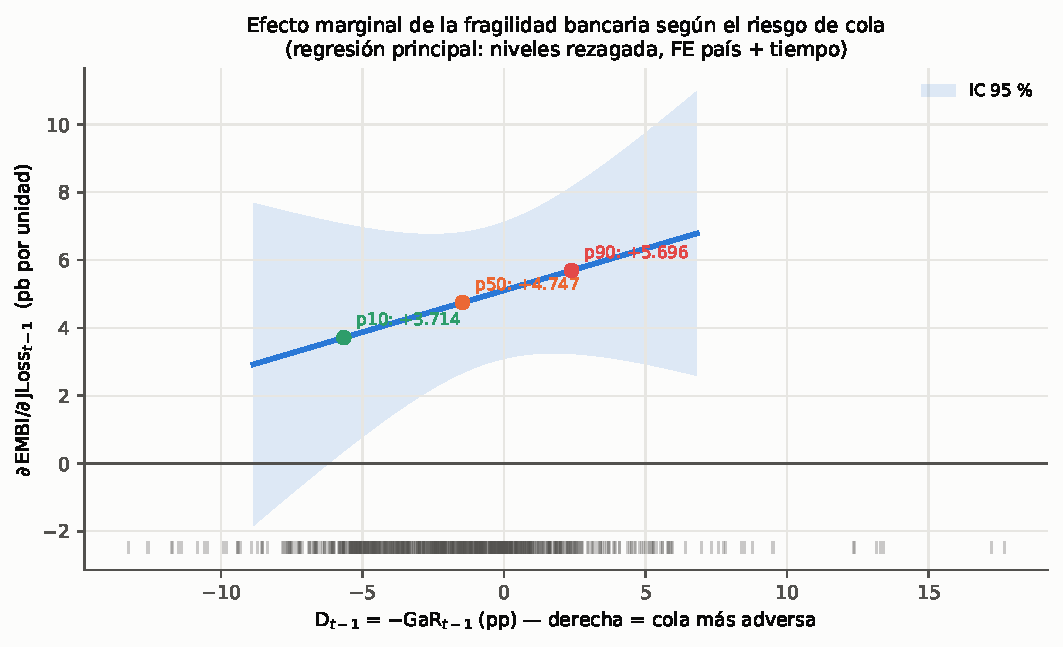
\includegraphics[width=0.82\textwidth]{fig_efecto_marginal_nivlag.pdf}
\caption[Efecto marginal de la fragilidad en niveles]{Efecto marginal de $JLoss_{t-1}$ sobre el spread en puntos básicos según el riesgo de cola $D_{t-1}$ (especificación en niveles rezagada, efectos fijos de país y de tiempo). Puntos: percentiles 10, 50 y 90 de $D$. Banda: IC 95\% (Driscoll--Kraay).}
\label{fig:efmarg-niv}
\end{figure}

\begin{figure}[htbp]
\centering
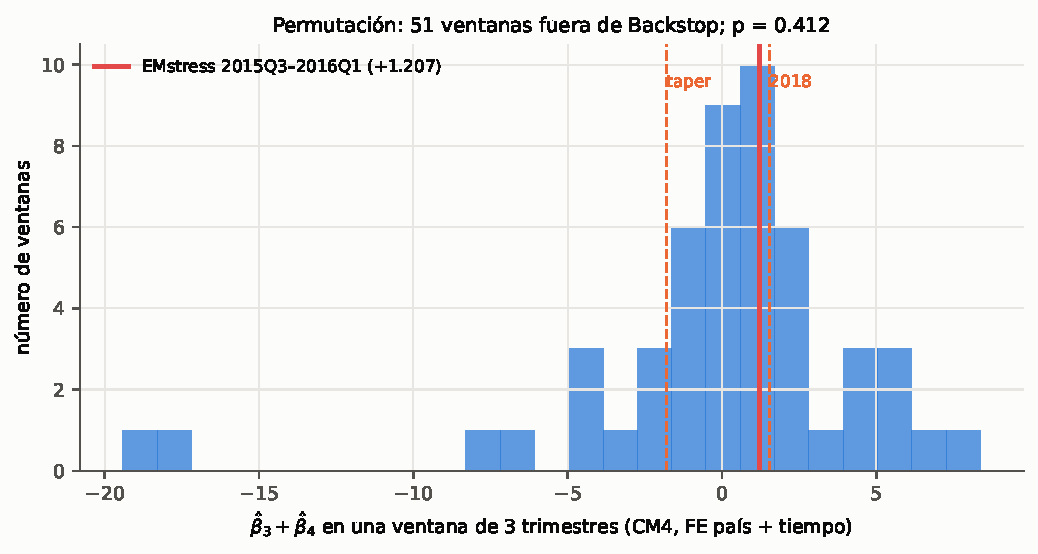
\includegraphics[width=0.82\textwidth]{fig_permutacion_emstress_arb_nivlag.pdf}
\caption[Prueba de permutación en niveles]{Prueba de permutación del episodio \textit{EMstress} en la especificación en niveles: distribución de $\hat\beta_3+\hat\beta_4$ (pb) al reemplazar 2015Q3--2016Q1 por cada ventana de tres trimestres consecutivos fuera de \textit{Backstop} (CM4, efectos fijos de país y de tiempo, seis controles).}
\label{fig:permutacion-niv}
\end{figure}


\section{Contabilidad del spread}
\label{sec:contabilidad}

La Figura~\ref{fig:contabilidad} descompone el cambio del spread en el choque de la pandemia (2019Q4 a 2020Q2) según la regresión principal, para las diez economías con ambos trimestres. El spread subió en promedio 63 log-puntos (×100) y el modelo predice 24: 21 del riesgo de cola, 10 de la fragilidad y $-7$ de la interacción. La mayor parte del salto corresponde al componente global común que absorben los efectos fijos de tiempo, y la parte atribuida a los determinantes domésticos hereda los límites de identificación de la Sección~\ref{sec:identificacion}. La Figura~\ref{fig:prima} traza el aporte del término de interacción al spread predicho: es pequeño en el trimestre típico (1,7\% del spread en valor absoluto) y cambia de signo según el episodio.

\begin{figure}[htbp]
\centering
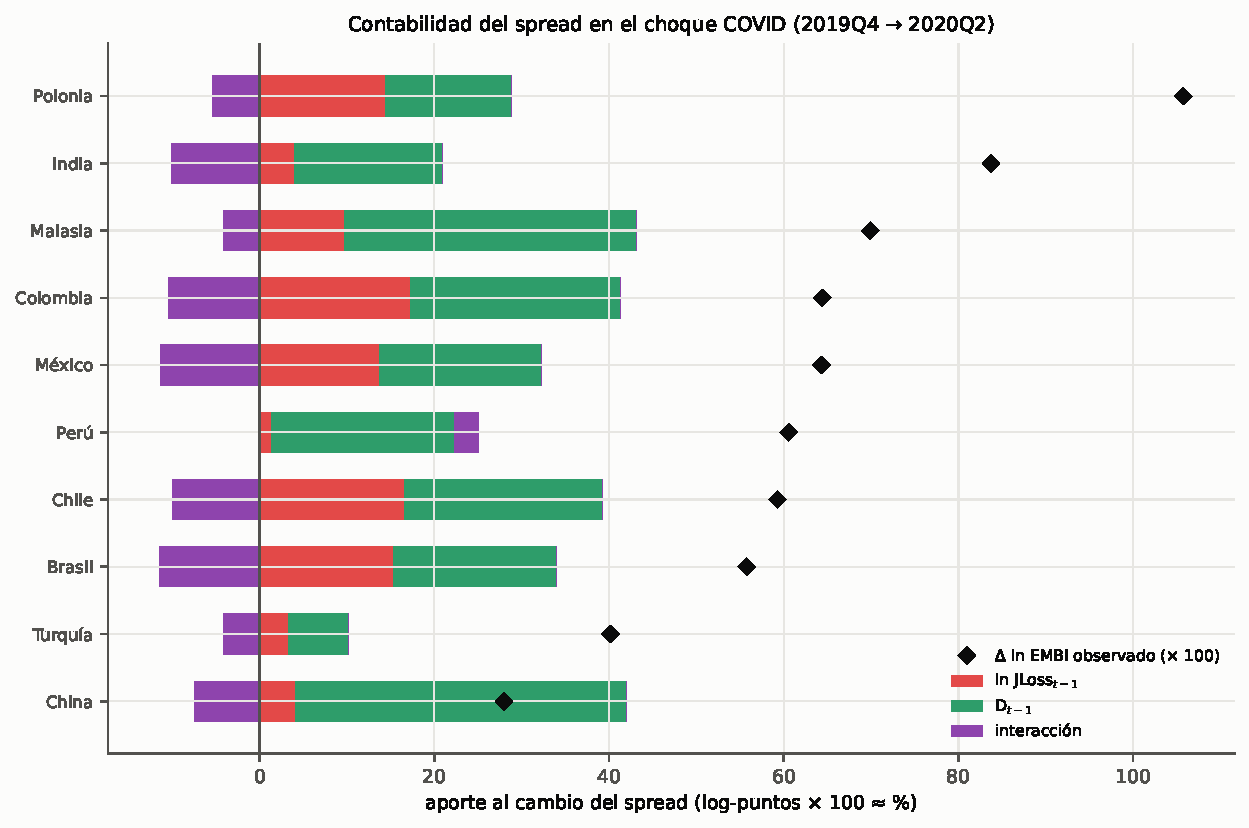
\includegraphics[width=0.85\textwidth]{fig_contabilidad_lnlag.pdf}
\caption[Contabilidad del spread en el choque COVID]{Aportes de $\ln JLoss_{t-1}$, $D_{t-1}$ y su interacción al cambio de $\ln$ EMBI entre 2019Q4 y 2020Q2 (log-puntos ×100), regresión principal, y cambio observado (rombos).}
\label{fig:contabilidad}
\end{figure}

\begin{figure}[htbp]
\centering
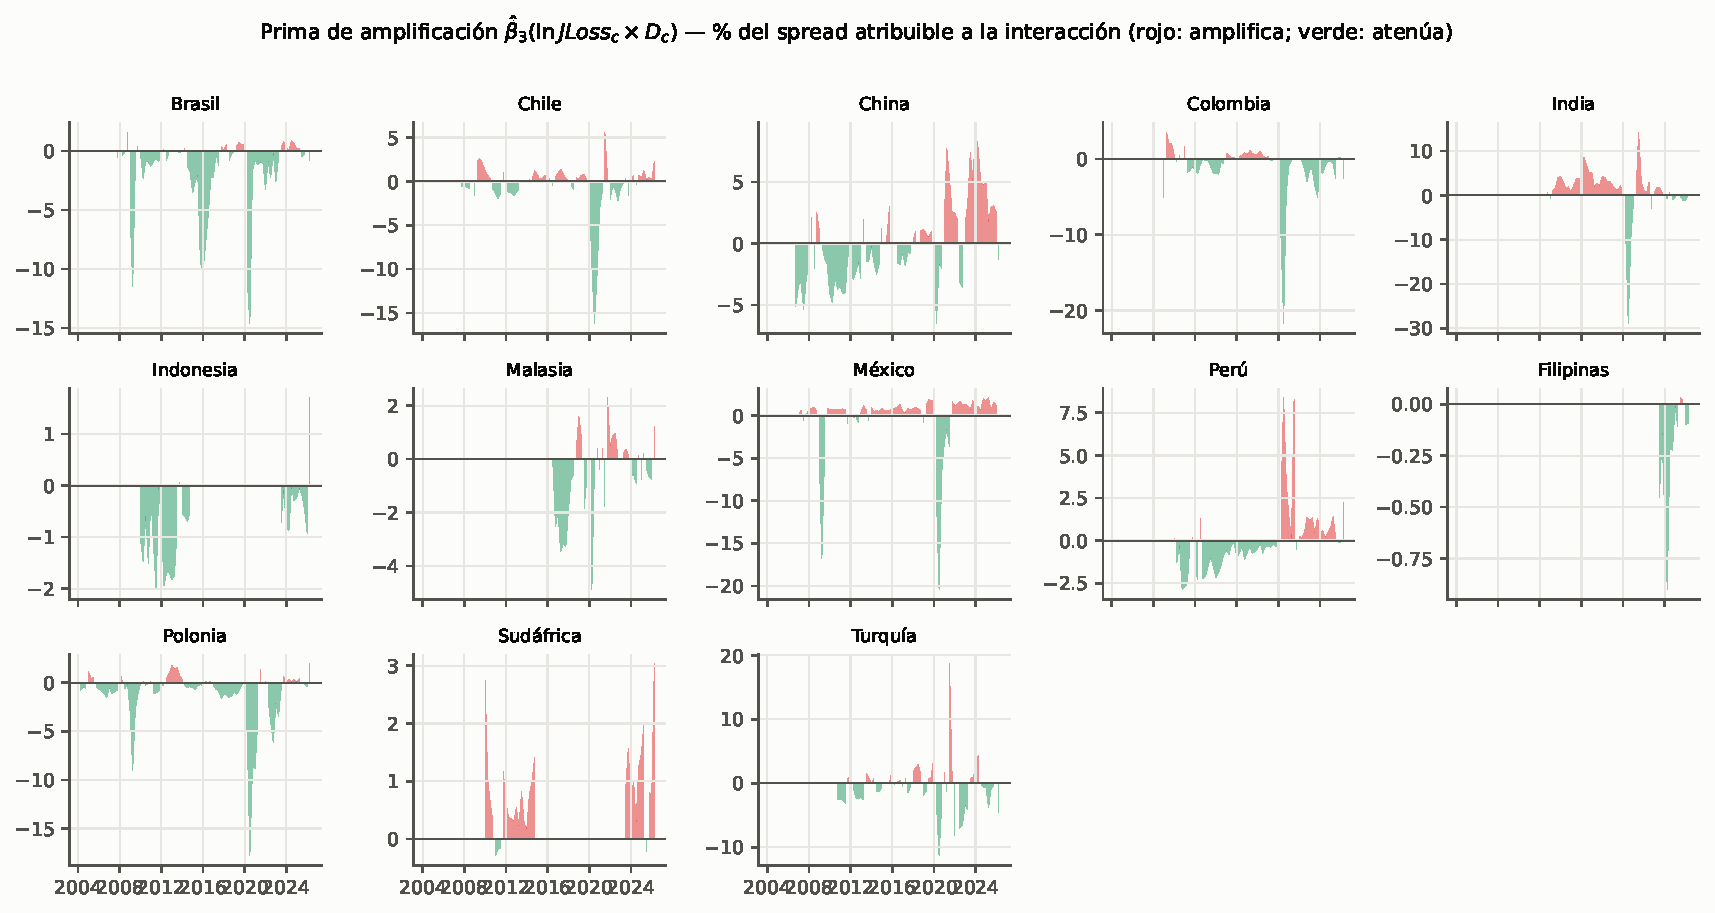
\includegraphics[width=\textwidth]{fig_prima_lnlag.pdf}
\caption[Prima de amplificación]{Aporte del término de interacción al spread predicho, $\hat\beta_3(\ln JLoss_c\times D_c)$, en \% del spread (regresión principal). Rojo: signo positivo; verde: negativo.}
\label{fig:prima}
\end{figure}

\section{Pendientes por país}
\label{sec:anexo-pendientes}

Las Tablas~\ref{tab:pendientes-pais} y~\ref{tab:pendientes-pais-cola} acompañan a la Sección~\ref{sec:loo-efectos}.

\begin{table}[htbp]
\centering
\small
\caption[Pendientes por país: fragilidad]{Pendientes por país y peso de cada economía en la fragilidad bancaria (regresión principal, log-log)}
\label{tab:pendientes-pais}
\begin{adjustbox}{max width=\linewidth}
\begin{tabular}{l c c c c c}
\toprule
País & $T$ & Pendiente del país & \% de la variación & Aporte a $\hat\beta_1$ & \% obs.\ en el piso \\
\midrule
Brasil & 75 & $-0{,}042$ & $12$ & $8$ & $0$ \\
Chile & 75 & $-0{,}009$ & $4$ & $0$ & $49$ \\
China & 79 & $-0{,}064$ & $23$ & $-17$ & $8$ \\
Colombia & 70 & $0{,}311^{***}$ & $10$ & $31$ & $26$ \\
Filipinas & 12 & $0{,}185^{*}$ & $1$ & $1$ & $0$ \\
India & 55 & $0{,}206^{***}$ & $9$ & $21$ & $0$ \\
Indonesia & 32 & $0{,}974^{***}$ & $1$ & $17$ & $34$ \\
Malasia & 40 & $0{,}355^{**}$ & $2$ & $9$ & $60$ \\
México & 77 & $-0{,}381^{***}$ & $9$ & $-27$ & $29$ \\
Perú & 66 & $0{,}118^{**}$ & $6$ & $7$ & $58$ \\
Polonia & 79 & $0{,}093$ & $5$ & $-15$ & $13$ \\
Sudáfrica & 32 & $-0{,}836^{***}$ & $1$ & $-3$ & $38$ \\
Turquía & 63 & $0{,}462^{***}$ & $17$ & $70$ & $2$ \\
\midrule
Promedio de grupo (13 países) & & $0{,}106$ & & & \\
\quad error estándar; $p$ & & $0{,}119$; $0{,}39$ & & & \\
Promedio de grupo ($T\geq40$, 10 países) & & $0{,}105$ & & & \\
Media ponderada por precisión & & $0{,}081$ & & & \\
Coeficiente agrupado (regresión principal) & 765 & $0{,}099^{***}$ & 100 & 100 & 23{,}7 \\
\bottomrule
\end{tabular}
\end{adjustbox}
\par\smallskip\parbox{0.95\linewidth}{\footnotesize \textit{Nota:} Pendientes por país: regresión de $\ln$ EMBI sobre $\ln JLoss_{t-1}$ y $D_{t-1}$ dentro de cada país, con las tres variables sin la media transversal de cada trimestre; se excluyen los diez trimestres en que solo un país tiene dato, todos de Polonia. Estrellas de las pendientes por país según errores HAC. ``\% de la variación'': participación del país en la variación de cada regresor que queda tras descontar los efectos fijos de país y de tiempo. ``Aporte'': parte del coeficiente agrupado que proviene de cada país en la descomposición exacta de Frisch--Waugh--Lovell, como porcentaje del coeficiente; los aportes suman 100 y pueden ser negativos. ``En el piso'': $JLoss_{t-1}$ a menos de un 2\% de $2{,}16$. Homogeneidad de pendientes: $\Delta=15{,}4$ ($p<0{,}001$) en la prueba de \citet{PesaranYamagata2008}; estadístico $Q$ de $128{,}7$ ($p<0{,}001$) para la fragilidad y $22{,}2$ ($p=0{,}035$) para el riesgo de cola. ***, ** y * indican significancia al 1\%, 5\% y 10\%. Fuente: \texttt{p30\_influencia\_paises.py}.}
\end{table}

\begin{table}[htbp]
\centering
\small
\caption[Pendientes por país: riesgo de cola]{Pendientes por país y peso de cada economía en el riesgo de cola (regresión principal, log-log)}
\label{tab:pendientes-pais-cola}
\begin{adjustbox}{max width=\linewidth}
\begin{tabular}{l c c c c}
\toprule
País & $T$ & Pendiente del país & \% de la variación & Aporte a $\hat\beta_2$ \\
\midrule
Brasil & 75 & $0{,}045^{***}$ & $13$ & $14$ \\
Chile & 75 & $0{,}004$ & $5$ & $0$ \\
China & 79 & $0{,}032$ & $17$ & $20$ \\
Colombia & 70 & $0{,}023$ & $9$ & $-3$ \\
Filipinas & 12 & $-0{,}005$ & $0$ & $0$ \\
India & 55 & $0{,}066^{***}$ & $5$ & $8$ \\
Indonesia & 32 & $-0{,}009$ & $1$ & $3$ \\
Malasia & 40 & $0{,}010$ & $10$ & $1$ \\
México & 77 & $0{,}022$ & $8$ & $-12$ \\
Perú & 66 & $0{,}044^{***}$ & $4$ & $-1$ \\
Polonia & 79 & $0{,}083^{*}$ & $16$ & $71$ \\
Sudáfrica & 32 & $-0{,}171^{**}$ & $1$ & $-9$ \\
Turquía & 63 & $0{,}002$ & $12$ & $7$ \\
\midrule
Promedio de grupo (13 países) & & $0{,}011$ & & \\
\quad error estándar; $p$ & & $0{,}017$; $0{,}52$ & & \\
Promedio de grupo ($T\geq40$, 10 países) & & $0{,}033^{***}$ & & \\
Media ponderada por precisión & & $0{,}023$ & & \\
Coeficiente agrupado (regresión principal) & 765 & $0{,}032^{**}$ & 100 & 100 \\
\bottomrule
\end{tabular}
\end{adjustbox}
\par\smallskip\parbox{0.95\linewidth}{\footnotesize \textit{Nota:} Pendientes por país: regresión de $\ln$ EMBI sobre $\ln JLoss_{t-1}$ y $D_{t-1}$ dentro de cada país, con las tres variables sin la media transversal de cada trimestre; se excluyen los diez trimestres en que solo un país tiene dato, todos de Polonia. Estrellas de las pendientes por país según errores HAC. ``\% de la variación'': participación del país en la variación de cada regresor que queda tras descontar los efectos fijos de país y de tiempo. ``Aporte'': parte del coeficiente agrupado que proviene de cada país en la descomposición exacta de Frisch--Waugh--Lovell, como porcentaje del coeficiente; los aportes suman 100 y pueden ser negativos. ``En el piso'': $JLoss_{t-1}$ a menos de un 2\% de $2{,}16$. Homogeneidad de pendientes: $\Delta=15{,}4$ ($p<0{,}001$) en la prueba de \citet{PesaranYamagata2008}; estadístico $Q$ de $128{,}7$ ($p<0{,}001$) para la fragilidad y $22{,}2$ ($p=0{,}035$) para el riesgo de cola. ***, ** y * indican significancia al 1\%, 5\% y 10\%. Fuente: \texttt{p30\_influencia\_paises.py}.}
\end{table}

\section{Otra medida del spread: el CDS soberano}
\label{sec:cds}

El EMBI es una de dos medidas habituales del riesgo soberano; la otra es la prima del \textit{credit default swap} (CDS) a cinco años, que no depende de la composición de un índice de bonos. El panel la trae para doce de las trece economías (India no tiene CDS en la muestra y Polonia solo catorce trimestres) y 635 observaciones; su correlación con el EMBI, en logaritmos, es de $0{,}83$. La Tabla~\ref{tab:cds} repite la regresión principal con el CDS como variable dependiente y, para separar el efecto de la medida del efecto de la muestra, con el EMBI sobre esas mismas 635 observaciones.

\begin{table}[htbp]
\centering
\small
\caption[Regresión principal con el CDS soberano]{Regresión principal con el CDS soberano a cinco años como variable dependiente (M4, efectos fijos de país y de tiempo, errores de Driscoll--Kraay)}
\label{tab:cds}
\begin{adjustbox}{max width=\linewidth}
\begin{tabular}{l ccc}
\toprule
 & Fragilidad ($\beta_1$) & Riesgo de cola ($\beta_2$) & Interacción ($\beta_3$) \\
\midrule
\multicolumn{4}{l}{\textit{Log-log}} \\
\quad EMBI, muestra principal ($N=765$) & $0{,}099^{***}$ & $0{,}032^{**}$ & $-0{,}011$ \\
\quad EMBI, muestra con CDS ($N=635$) & $0{,}114^{***}$ & $0{,}008$ & $0{,}010$ \\
\quad CDS ($N=635$) & $0{,}206^{***}$ & $0{,}013$ & $0{,}016^{**}$ \\
\addlinespace
\multicolumn{4}{l}{\textit{Niveles (pb)}} \\
\quad EMBI, muestra principal ($N=765$) & $4{,}73^{***}$ & $3{,}24$ & $0{,}25$ \\
\quad EMBI, muestra con CDS ($N=635$) & $5{,}72^{***}$ & $-0{,}30$ & $0{,}75^{**}$ \\
\quad CDS ($N=635$) & $7{,}45^{***}$ & $2{,}64$ & $0{,}89^{**}$ \\
\bottomrule
\end{tabular}
\end{adjustbox}
\par\smallskip\parbox{0.95\linewidth}{\footnotesize \textit{Nota:} Regresores rezagados un trimestre y centrados. La muestra con CDS tiene doce economías: no incluye a India y de Polonia solo catorce trimestres. ***, ** y * indican significancia al 1\%, 5\% y 10\%. Fuente: \texttt{p24\_robustez\_medicion.py}.}
\end{table}

La asociación de la fragilidad bancaria no depende de cómo se mida el spread: con el CDS es positiva, significativa al 1\% y de magnitud mayor ($0{,}21$ frente a $0{,}11$ con el EMBI sobre la misma muestra). La del riesgo de cola, en cambio, no es significativa en esta muestra con ninguna de las dos medidas ($0{,}013$ con el CDS y $0{,}008$ con el EMBI), de modo que lo que la debilita no es la medida sino la muestra, que casi no incluye a Polonia: es el mismo resultado de la Tabla~\ref{tab:pendientes-pais-cola} por otro camino. La interacción es positiva en esta muestra y significativa al 5\% con el CDS, solo con Driscoll--Kraay; como la muestra con CDS se parece al grupo de once economías de la Sección~\ref{sec:robustez-heterogeneidad}, el resultado hereda las salvedades de esa agrupación.

\section{Solapamiento del riesgo de cola con las variables financieras}
\label{sec:robustez-solapamiento}

La Tabla~\ref{tab:solapamiento} reporta las pruebas de la Sección~\ref{sec:est-solapamiento}. Los factores financieros globales explican el 34\% de la variación del riesgo de cola dentro de cada país, y los efectos fijos de país y de tiempo, el 82\%; tras descontarlos, la correlación parcial entre $D_{t-1}$ y $\ln JLoss_{t-1}$ es de 0,26, lo que equivale a un factor de inflación de varianza de 1,07: los dos riesgos comparten poca variación y no hay un problema de colinealidad.

\begin{table}[htbp]
\centering
\small
\caption[Solapamiento del riesgo de cola con las variables financieras]{Riesgo de cola limpio de las variables financieras (M4; errores de Driscoll--Kraay)}
\label{tab:solapamiento}
\begin{adjustbox}{max width=\linewidth}
\begin{tabular}{l ccc}
\toprule
 & $\beta_1$ (fragilidad) & $\beta_2$ (riesgo de cola) & $\beta_3$ (interacción) \\
\midrule
\multicolumn{4}{l}{\textit{Efectos fijos de país y de tiempo}} \\
\quad Especificación principal & $0{,}099^{***}$ & $0{,}032^{**}$ & $-0{,}011$ \\
\quad $D$ limpio de los factores globales & $0{,}110^{***}$ & $0{,}033^{**}$ & $-0{,}016^{**}$ \\
\quad $D$ limpio de $\ln JLoss$ & $0{,}125^{***}$ & $0{,}035^{**}$ & $-0{,}023$ \\
\addlinespace
\multicolumn{4}{l}{\textit{Solo efectos fijos de país}} \\
\quad Sin limpiar & $0{,}152^{***}$ & $0{,}017^{*}$ & $-0{,}006$ \\
\quad $D$ limpio de los factores globales & $0{,}191^{***}$ & $0{,}013$ & $-0{,}013$ \\
\addlinespace
\multicolumn{4}{l}{\textit{$GaR$ estimado en muestra completa (efectos fijos de país y de tiempo)}} \\
\quad Con el bloque bursátil del FCI & $0{,}096^{***}$ & $0{,}039^{**}$ & $-0{,}006$ \\
\quad Sin el bloque bursátil del FCI & $0{,}096^{***}$ & $0{,}045^{**}$ & $-0{,}004$ \\
\bottomrule
\end{tabular}
\end{adjustbox}
\par\smallskip\parbox{0.95\linewidth}{\footnotesize \textit{Nota:} ``Limpio'' es el residuo de regresar $D_{t-1}$ sobre los factores globales (VIX, tasa del Tesoro a diez años, spread de alto rendimiento y \textit{on/off-the-run}, con efectos fijos de país) o sobre $\ln JLoss_{t-1}$ (con efectos fijos de país y de tiempo). Las dos últimas filas usan el $GaR$ estimado una sola vez sobre toda la muestra, con y sin el bloque bursátil del FCI ($N=773$); las demás, la muestra principal ($N=765$). ***, ** y * indican significancia al 1\%, 5\% y 10\%. Fuente: \texttt{p18\_solapamiento\_gar.py}.}
\end{table}

Con efectos fijos de país y de tiempo, limpiar el riesgo de cola de los factores globales o de la propia fragilidad deja su coeficiente prácticamente igual ($0{,}033$ y $0{,}035$ frente a $0{,}032$): los efectos fijos de tiempo ya absorben el componente global. Reconstruir el $GaR$ sin el bloque bursátil del FCI ---el que comparte información con $JLoss$--- tampoco cambia nada: la serie resultante correlaciona 0,98 con la que lo incluye y su coeficiente es $0{,}045$ frente a $0{,}039$. El riesgo de cola no es, por tanto, un reflejo de las variables financieras que ya están en la regresión. La prueba sí acota el resultado en una dirección: con solo efectos fijos de país, donde los factores globales no están absorbidos, el riesgo de cola limpio de ellos deja de ser significativo ($0{,}013$, $p=0{,}17$). Parte de su asociación con el spread es global, y es la especificación con efectos fijos de tiempo la que aísla su componente doméstico.

\section{Figuras y tablas complementarias}
\label{sec:anexo-complementarias}

Figuras y tablas de detalle de las Secciones~\ref{sec:loo-efectos}, \ref{sec:aporte-cola}, \ref{sec:robustez-resiliencia}, \ref{sec:crisis-interaccion}, \ref{sec:participacion-extranjera} e \ref{sec:identificacion}.

\begin{figure}[htbp]
\centering
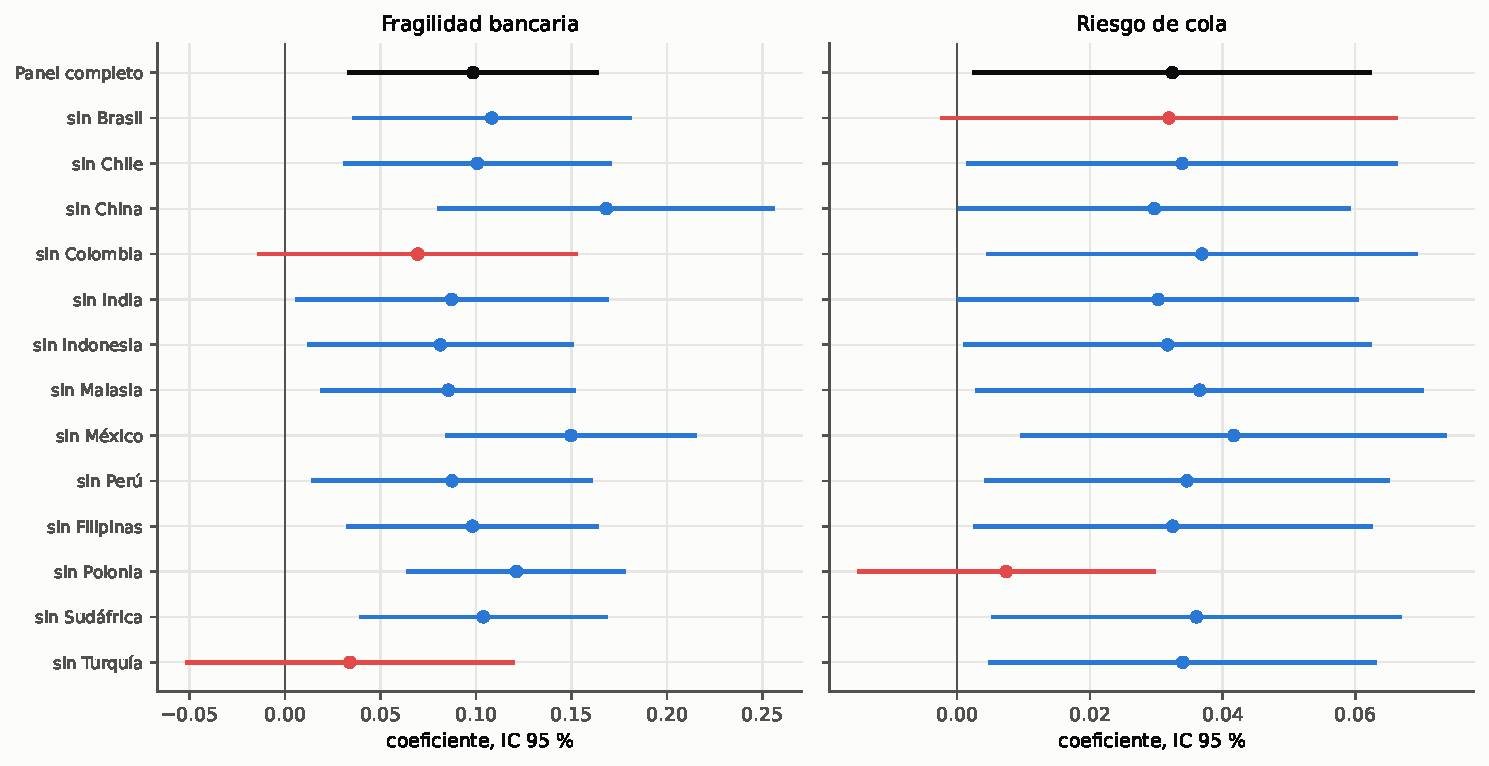
\includegraphics[width=\textwidth]{fig_loo_efectos_lnlag.pdf}
\caption[\textit{Leave-one-country-out} de los efectos de cada riesgo]{Elasticidad de la fragilidad ($\hat\beta_1$, izquierda) y semielasticidad del riesgo de cola ($\hat\beta_2$, derecha) de la regresión principal excluyendo cada país (IC 95\%, Driscoll--Kraay). En rojo, las exclusiones en que el coeficiente deja de ser significativo al 5\%.}
\label{fig:loo-efectos}
\end{figure}

\begin{figure}[htbp]
\centering
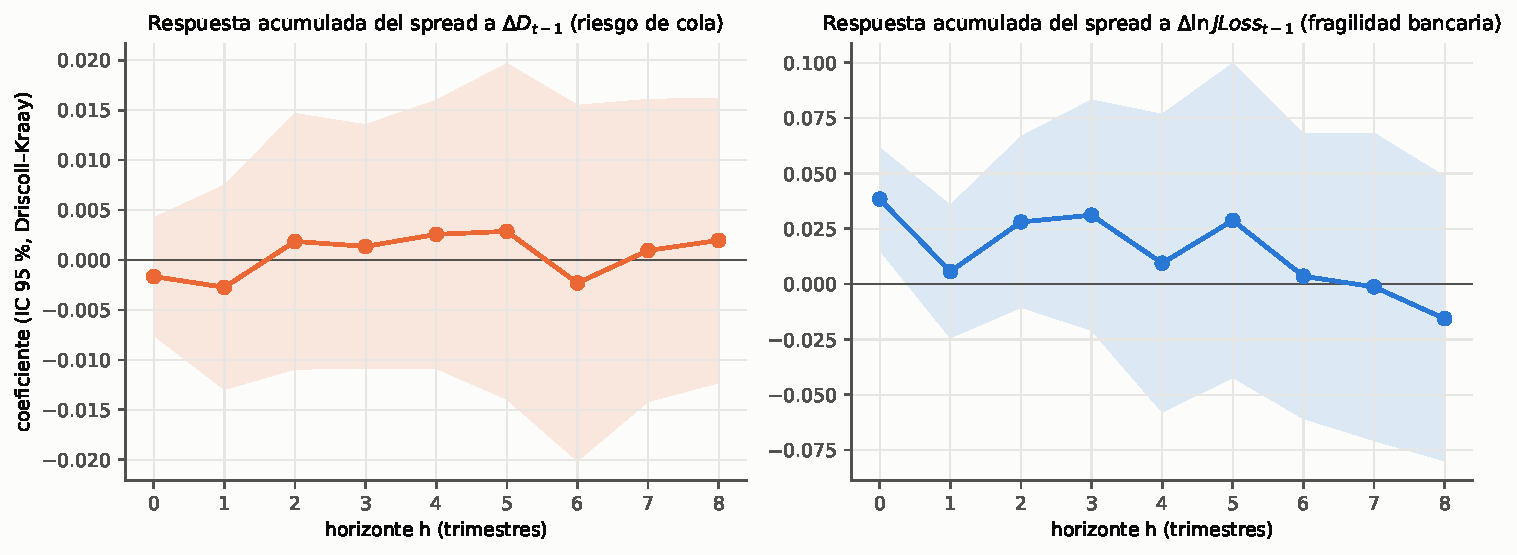
\includegraphics[width=\textwidth]{fig_aporte_cola_lnlag.pdf}
\caption[Proyecciones locales acumuladas de cada riesgo]{Respuesta acumulada de $\ln$ EMBI entre $t-1$ y $t+h$ al cambio del riesgo de cola (izquierda) y al de la fragilidad (derecha) en $t-1$, con efectos fijos de país y de tiempo. Banda: IC 95\% (Driscoll--Kraay con ancho de banda creciente en el horizonte).}
\label{fig:aporte-cola}
\end{figure}

\begin{figure}[htbp]
\centering
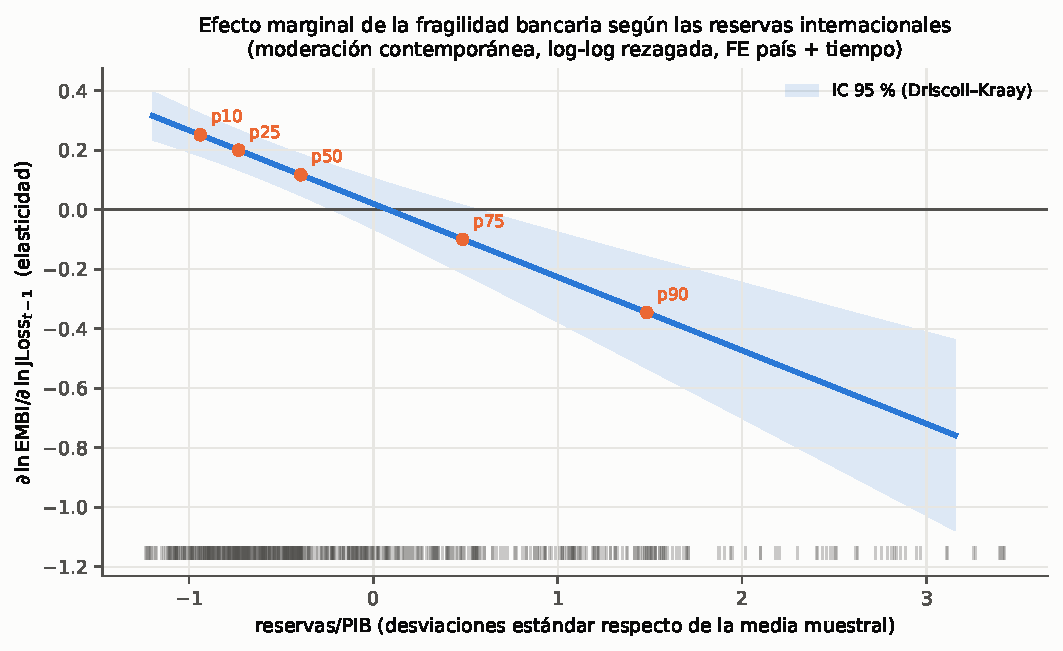
\includegraphics[width=0.82\textwidth]{fig_reservas_efecto_marginal_lnlag.pdf}
\caption[Elasticidad de la fragilidad según las reservas]{Elasticidad del spread a $JLoss_{t-1}$ que implica la interacción lineal con las reservas/PIB (contemporáneas, estandarizadas). Puntos: percentiles 10, 25, 50, 75 y 90 de las reservas. Banda: IC 95\% (Driscoll--Kraay). Marcas inferiores: observaciones.}
\label{fig:reservas-efmarg}
\end{figure}

\begin{figure}[htbp]
\centering
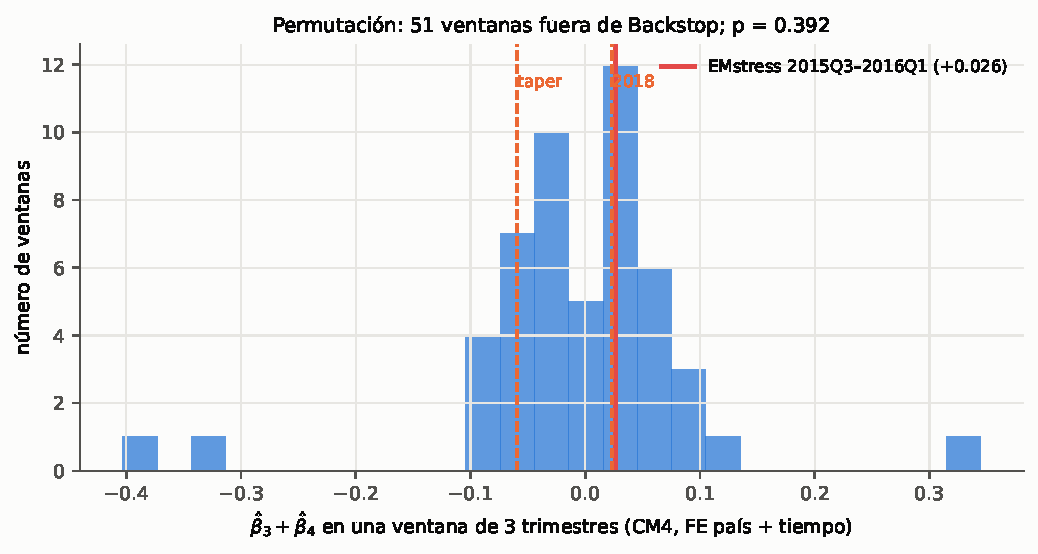
\includegraphics[width=0.82\textwidth]{fig_permutacion_emstress_arb.pdf}
\caption[Prueba de permutación del episodio EMstress]{Distribución de $\hat\beta_3+\hat\beta_4$ al reemplazar el episodio \textit{EMstress} por cada ventana de tres trimestres consecutivos fuera de \textit{Backstop} (CM4, efectos fijos de país y de tiempo, seis controles). Línea roja: 2015Q3--2016Q1; líneas discontinuas: \textit{taper tantrum} y 2018.}
\label{fig:permutacion}
\end{figure}

\begin{figure}[htbp]
\centering
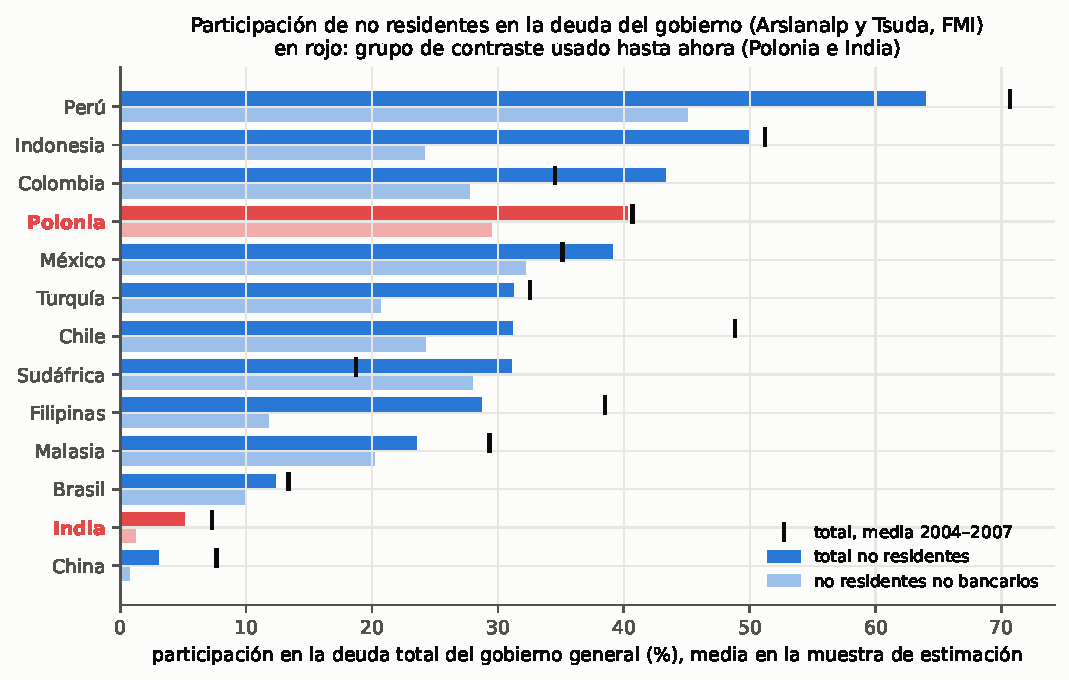
\includegraphics[width=0.85\textwidth]{fig_participacion_extranjera.pdf}
\caption[Participación de no residentes en la deuda del gobierno]{Participación de no residentes en la deuda total del gobierno general, media en la muestra de estimación (barra oscura: total; barra clara: no residentes no bancarios; marca: media del total en 2004--2007). En rojo, Polonia e India, la agrupación \textit{ex post} de la Sección~\ref{sec:robustez-heterogeneidad}. Fuente: \citet{ArslanalpTsuda2014}, versión de mayo de 2026.}
\label{fig:participacion}
\end{figure}

\begin{figure}[htbp]
\centering
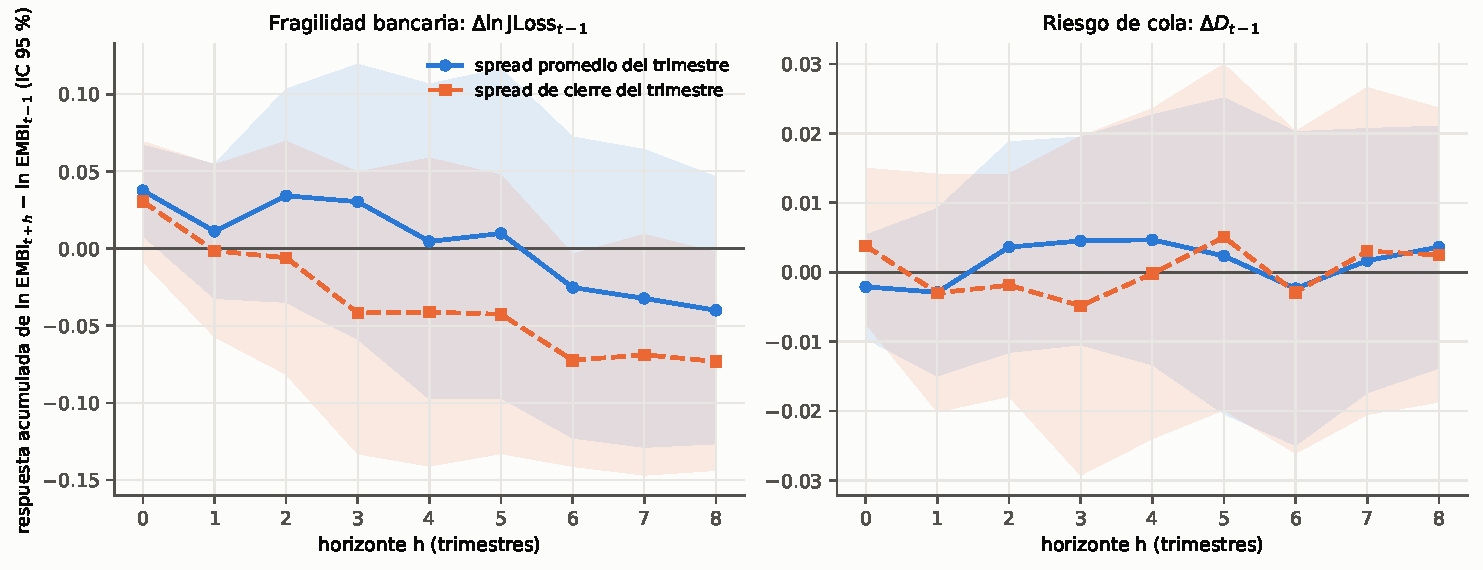
\includegraphics[width=\textwidth]{fig_lp_acumulada_lnlag.pdf}
\caption[Proyecciones locales acumuladas con el spread promedio y de cierre]{Proyecciones locales acumuladas: respuesta de $\ln\mathrm{EMBI}_{t+h}-\ln\mathrm{EMBI}_{t-1}$ al cambio de la fragilidad (izquierda) y del riesgo de cola (derecha) en $t-1$, con el spread promedio del trimestre (línea continua) y con el spread de cierre (línea discontinua). Dos rezagos de los cambios de las tres variables y efectos fijos de país y de tiempo. Banda: IC 95\% (Driscoll--Kraay).}
\label{fig:lp-acumulada}
\end{figure}

\begin{table}[htbp]
\centering
\small
\caption[Participación extranjera por país]{Participación de no residentes en la deuda del gobierno general, por país (\% de la deuda total)}
\label{tab:participacion-ranking}
\begin{adjustbox}{max width=\linewidth}
\begin{tabular}{l ccccc}
\toprule
 & \multicolumn{3}{c}{Media en la muestra de estimación} & Total, & Total, \\
\cmidrule(lr){2-4}
País & Total & No bancos & Sector oficial & media 2004--2007 & mínimo--máximo \\
\midrule
Perú & $64{,}0$ & $45{,}0$ & $19{,}0$ & $70{,}7$ & $53$--$74$ \\
Indonesia & $50{,}1$ & $24{,}2$ & $24{,}2$ & $51{,}2$ & $34$--$61$ \\
Colombia & $43{,}3$ & $27{,}7$ & $15{,}4$ & $34{,}5$ & $27$--$57$ \\
Polonia & $40{,}3$ & $29{,}5$ & $10{,}9$ & $40{,}7$ & $27$--$55$ \\
México & $39{,}1$ & $32{,}2$ & $6{,}8$ & $35{,}1$ & $23$--$56$ \\
Turquía & $31{,}3$ & $20{,}6$ & $8{,}4$ & $32{,}6$ & $11$--$53$ \\
Chile & $31{,}2$ & $24{,}2$ & $5{,}2$ & $48{,}9$ & $17$--$54$ \\
Sudáfrica & $31{,}0$ & $28{,}0$ & $1{,}3$ & $18{,}7$ & $16$--$41$ \\
Filipinas & $28{,}7$ & $11{,}8$ & $16{,}9$ & $38{,}5$ & $25$--$45$ \\
Malasia & $23{,}5$ & $20{,}2$ & $3{,}3$ & $29{,}3$ & $19$--$35$ \\
Brasil & $12{,}4$ & $10{,}0$ & $2{,}1$ & $13{,}4$ & $10$--$19$ \\
India & $5{,}1$ & $1{,}2$ & $3{,}9$ & $7{,}3$ & $4$--$9$ \\
China & $3{,}0$ & $0{,}8$ & $2{,}2$ & $7{,}7$ & $2$--$10$ \\
\bottomrule
\end{tabular}
\end{adjustbox}
\par\smallskip\parbox{0.95\linewidth}{\footnotesize \textit{Nota:} Países ordenados por la participación total. ``No bancos'' es el moderador primario de la Tabla~\ref{tab:participacion}. El total incluye además la tenencia de bancos extranjeros, que no supera el 2,2\% en ninguna economía. Fuente: \texttt{p26\_participacion\_extranjera.py}, con datos de \citet{ArslanalpTsuda2014}.}
\end{table}

\begin{table}[htbp]
\centering
\small
\caption[Inferencia: errores alternativos, tamaño y potencia]{$p$-valores según el estimador de la varianza, y frecuencia de rechazo al 5\% nominal en la simulación (fragilidad / riesgo de cola)}
\label{tab:inferencia}
\begin{adjustbox}{max width=\linewidth}
\begin{tabular}{l ccc ccc}
\toprule
 & \multicolumn{3}{c}{$p$-valor en los datos} & Tamaño & Potencia & Tamaño \\
 & $\beta_1$ & $\beta_2$ & $\beta_3$ & (proceso B) & (proceso B) & (proceso C, centrado) \\
\midrule
\multicolumn{7}{l}{\textit{Niveles (regresión principal)}} \\
\quad Driscoll--Kraay & $0{,}003$ & $0{,}033$ & $0{,}11$ & $28\%$ / $21\%$ & $70\%$ / $77\%$ & $18\%$ / $18\%$ \\
\quad Driscoll--Kraay, banda larga y valores críticos \textit{fixed-b} & $0{,}030$ & $0{,}11$ & $0{,}18$ & $15\%$ / $11\%$ & $56\%$ / $66\%$ & $9\%$ / $10\%$ \\
\quad \textit{Cluster} por país, $t(12)$ & $0{,}28$ & $0{,}14$ & $0{,}53$ & $9\%$ / $8\%$ & $44\%$ / $70\%$ & $6\%$ / $14\%$ \\
\quad \textit{Wild cluster bootstrap} por país & $0{,}33$ & $0{,}20$ & $0{,}89$ & $6\%$ / $7\%$ & $35\%$ / $67\%$ & $5\%$ / $12\%$ \\
\addlinespace
\multicolumn{7}{l}{\textit{Primeras diferencias (spread promedio)}} \\
\quad Driscoll--Kraay & $0{,}002$ & $0{,}53$ & $0{,}31$ & $5\%$ / $6\%$ & $87\%$ / --- & --- \\
\quad \textit{Cluster} por país, $t(12)$ & $0{,}011$ & $0{,}25$ & $0{,}45$ & $6\%$ / $9\%$ & $84\%$ / --- & --- \\
\quad \textit{Wild cluster bootstrap} por país & $0{,}007$ & $0{,}24$ & --- & $6\%$ / $6\%$ & $81\%$ / --- & --- \\
\bottomrule
\end{tabular}
\end{adjustbox}
\par\smallskip\parbox{0.95\linewidth}{\footnotesize \textit{Nota:} ``Tamaño'': frecuencia de rechazo cuando la hipótesis nula es cierta; un contraste bien calibrado rechazaría el 5\%. ``Potencia'': frecuencia de rechazo cuando el coeficiente verdadero es el estimado. Proceso B: residuos restringidos con un autorregresivo de orden dos por país, remuestreados por fecha en bloques de cuatro trimestres, regresores fijos. Proceso C: vector autorregresivo de panel con retroalimentación; ``centrado'' contrasta contra la media del estimador bajo la hipótesis nula, de modo que mide solo la calibración del error estándar y no el sesgo de retroalimentación. \textit{Fixed-b}: ancho de banda de $0{,}2\,T$ y valores críticos de \citet{KieferVogelsang2005}. En primeras diferencias la potencia se reporta para la fragilidad. 1\,000 simulaciones y 199 réplicas internas. Con el proceso A el \textit{wild bootstrap} rechaza una hipótesis nula cierta el 9\% y el 16\% de las veces, y su potencia es 15\% y 37\%. Fuente: \texttt{p29\_simulacion\_v2.py}.}
\end{table}
